\section{Design and Implementation}

\subsection{Overall power management design}

The aims set out for the preliminary design were to incorporate new batteries into Tiberius III, use more efficient motors, reduce the weight and improve the monitoring and control of the power from the various devices and motors that Tiberius would use.  These features were implemented with varying degrees of success.  
The weight was dramatically reduced due to the restructuring of the chassis by removing about half of the aluminium extrusion, the various mountings and battery holders were all 3D printed using lightweight PLA and the batteries themselves were also significantly lighter than the previous versions.  However, Tiberius III ended up being about 10Kg heavier than Tiberius II due to the additional hardware including robotic arm which added quite a bit of weight.  
\newline
The control Raspberry Pi had a power monitoring mbed which allowed it to monitor the power usage and used capacity of the batteries and an Arduino to control relays which could be used to turn off the Kinect 2 sensor and processor, the robotic arm and even the ability to shut down the motors if necessary. Figure \ref{fig:power} shows the initial design of the power system for Tiberius III. This design has changed slightly with the sensors not being turned off due to how little power they used and the spare relay being used to control 12v to the stepper driver instead.

  

\begin{figure}[!htb]
\begin{center}
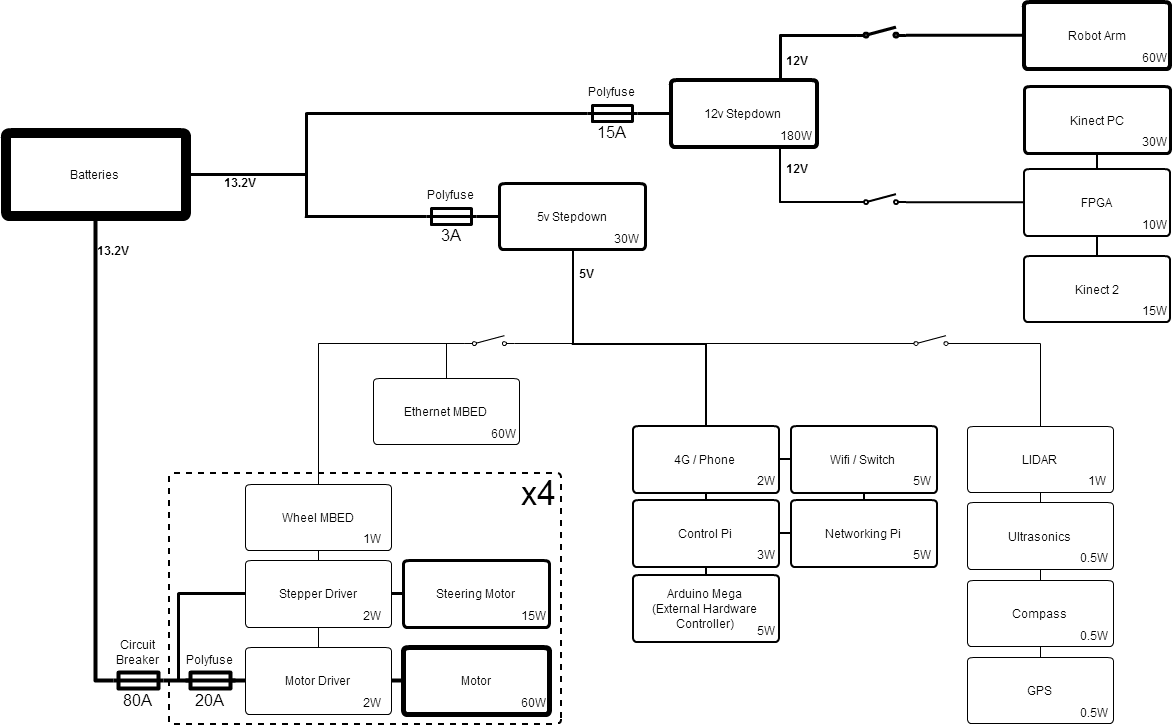
\includegraphics[width=15cm]{power.png}
\end{center}
\caption{Initial Power Management Design}
\label{fig:power}
\end{figure}

\subsection{Power monitoring and usage}
Two specialised current sensing boards were used to measure the current being used from the batteries as well as the voltage. The boards were connected to an mbed which calculated the current power consumption, and total used power in amp-hours and watt-hours.

This monitoring can then be used to work out if Tiberius can complete a mission without running out of power.
